\documentclass[a4paper, 10pt]{article}
\usepackage[utf8]{inputenc}
\usepackage[T1]{fontenc}
\usepackage[margin=2.5cm]{geometry}
\usepackage{graphicx}
\usepackage{url}
\usepackage{booktabs}
\usepackage{amsmath}
\usepackage{float}
\usepackage{xcolor}
\usepackage{listings}
\usepackage{subcaption}
\usepackage{pgfplots}
\usepackage{hyperref}
\pgfplotsset{compat=1.18}
\usepackage{microtype}
\setlength{\emergencystretch}{3em}

\lstdefinelanguage{erlang}{
  morekeywords={case,of,end,if,receive,after,when,fun,spawn,true,false},
  sensitive=true,
  morecomment=[l]{\%},
  morestring=[b]",
}
\lstset{
  language=erlang,
  basicstyle=\ttfamily\footnotesize,
  keywordstyle=\bfseries,
  commentstyle=\itshape\color{gray},
  breaklines=true,
  frame=single,
  columns=fullflexible,
}

\pgfplotsset{
  paxy/.style={
    width=0.48\textwidth, height=5.2cm,
    grid=major, grid style={gray!25},
    legend style={font=\footnotesize, draw=none, fill=none},
    legend cell align=left,
    tick label style={font=\footnotesize},
    label style={font=\footnotesize},
    mark size=1.6pt,
  },
}

%opening
\title{Seminar Report: Paxy}
\author{
  \textbf{Shahroz Ali} -- shahroz.ali@estudiantat.upc.edu \\
  \textbf{Jose Ricardo Arias Perez} -- jose.ricardo.arias@estudiantat.upc.edu \\[4pt]
}
\date{\normalsize November 22nd, 2026}

\begin{document}

\maketitle

\section{Introduction}

This seminar implements Paxos, the classic protocol for \emph{consensus}: a group of processes that communicate only by messages, which can be delayed, lost or sent to processes that crash, must agree on a single value. We implement the \emph{proposer} and \emph{acceptor} roles in Erlang (\emph{Paxy}). Five acceptors and three proposers agree on a colour. We then study how message delays, missing \texttt{sorry} messages, lost messages and the number of processes affect the time and the number of rounds needed. We also make the system distributed over several Erlang nodes, make the acceptors survive crashes, and use \texttt{sorry} messages to abort early.

% \paragraph{Methodology.} To get repeatable numbers we wrote a headless benchmark (\texttt{experiments/bench.erl}). It runs the \emph{unmodified} \texttt{acceptor} and \texttt{proposer} modules, but replaces the wx panels with a process that ignores every message. Each experimental variant (delay, drop ratio, timeout, \dots) is selected with a compile-time flag (e.g.\ \texttt{erlc -Dpromise\_delay=500}), so the default build is the normal code. Every configuration was run 20 times. In each trial all proposers start at the same time (initial sleep 0), which is the worst case for contention. A trial reaches \emph{consensus} when every proposer has decided within 60\,s. We report the mean time until the last proposer decides, and the number of rounds that proposer needed (the first round, \texttt{\{0,Name\}}, counts as round~1). Unless stated otherwise: 5 acceptors, 3 proposers, timeout 2000\,ms, and the \emph{basic} proposer of the statement (\texttt{sorry} messages do not abort a ballot). \texttt{experiments/run\_experiments.sh} reproduces all 62 configurations (1240 trials) in about 18 minutes. \textbf{In all 1240 trials, all proposers that decided chose the same value}: none of the perturbations below ever broke safety.

\paragraph{Baseline:} The three proposers need on average 2.8 rounds and \textbf{3.7\,s} to decide. Almost all of that time is spent waiting for timeouts. The proposer with the highest round wins at once, but every other proposer receives \texttt{sorry} messages for its round. The basic code ignores them, so the losing proposers only notice the failure after the 2\,s timeout, and this happens about twice per trial.

\section{Experiments and Questions}

\subsection{Message delays}

\textbf{Experiment.} The acceptor delays each \texttt{promise}, \texttt{vote}, or both, by a random time in $[1, D]$\,ms (\texttt{timer:send\_after}). Figure~\ref{fig:delay} and Table~\ref{tab:timeout} show the results. All 20 trials reached consensus in every configuration.

\begin{figure}[H]
\centering
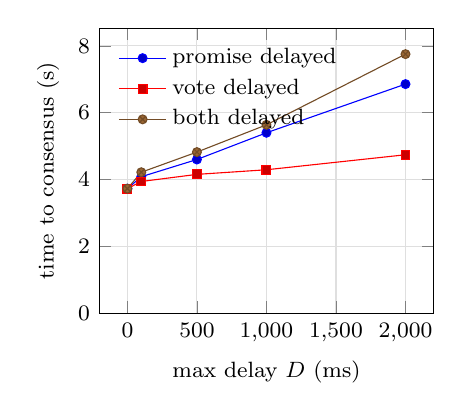
\begin{tikzpicture}
\begin{axis}[paxy, xlabel={max delay $D$ (ms)}, ylabel={time to consensus (s)},
             xtick={0,500,1000,1500,2000}, legend pos=north west, ymin=0]
\addplot coordinates {(0,3.727) (100,4.084) (500,4.599) (1000,5.399) (2000,6.856)};
\addplot coordinates {(0,3.727) (100,3.941) (500,4.154) (1000,4.292) (2000,4.741)};
\addplot coordinates {(0,3.727) (100,4.218) (500,4.821) (1000,5.637) (2000,7.753)};
\legend{promise delayed, vote delayed, both delayed}
\end{axis}
\end{tikzpicture}\hfill
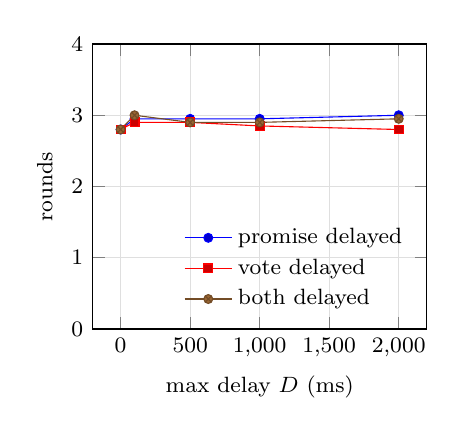
\begin{tikzpicture}
\begin{axis}[paxy, xlabel={max delay $D$ (ms)}, ylabel={rounds},
             xtick={0,500,1000,1500,2000}, ymin=0, ymax=4, legend pos=south east]
\addplot coordinates {(0,2.80) (100,2.95) (500,2.95) (1000,2.95) (2000,3.00)};
\addplot coordinates {(0,2.80) (100,2.90) (500,2.90) (1000,2.85) (2000,2.80)};
\addplot coordinates {(0,2.80) (100,3.00) (500,2.90) (1000,2.90) (2000,2.95)};
\legend{promise delayed, vote delayed, both delayed}
\end{axis}
\end{tikzpicture}
\caption{Message delays with the default timeout of 2000\,ms (mean of 20 trials).}
\label{fig:delay}
\end{figure}

\begin{table}[H]
\centering
\begin{tabular}{rrrrrrr}
\toprule
timeout (ms) & 250 & 500 & 750 & 1000 & 2000 & 4000 \\
\midrule
time to consensus (s) & 1.89 & 1.97 & 2.40 & 2.99 & 4.82 & 8.79 \\
rounds (mean / max)  & 3.85 / 6 & 2.85 / 3 & 2.85 / 3 & 3.05 / 4 & 2.90 / 3 & 2.95 / 3 \\
\bottomrule
\end{tabular}
\caption{Timeout sweep with both \texttt{promise} and \texttt{vote} delayed by up to 500\,ms.}
\label{tab:timeout}
\end{table}

\textbf{Question.} The algorithm always terminates, and with the default timeout the number of rounds does not grow. Only the time grows, roughly linearly with $D$. Delaying \texttt{promise} costs more than delaying \texttt{vote}, because every ballot, including the ones that fail, waits for promises, while only the ballots that reach phase~2 wait for votes.

% Rounds do not increase even when $D$ equals the timeout because (i) a proposer only needs the 3 fastest of 5 replies, and (ii) the \texttt{after} clause in \texttt{collect}/\texttt{vote} restarts on every received message, so a phase aborts only if the \emph{gap} between two consecutive replies exceeds the timeout. Delays only cause extra rounds when they are of the order of the timeout or larger. With delays up to 500\,ms and a timeout of 250\,ms, the mean rises to 3.85 rounds (max 6): proposers give up on ballots that would have succeeded, and they still reach consensus.

The timeout has a much stronger effect on the time than the delays (Table~\ref{tab:timeout}). Most of the time is spent by losing proposers waiting for a timeout, so a shorter timeout makes consensus much faster. The trade-off is that a timeout below the typical message delay causes premature aborts, more rounds and more traffic. If the timeout is far below the delay, no quorum is ever collected in time and the system livelocks. The timeout should therefore be somewhat above the expected round-trip time.

\subsection{\texttt{sorry} messages}

\textbf{Experiment.} We compiled the acceptor with \texttt{-Dno\_sorry}, which suppresses both kinds of \texttt{sorry} message.

\begin{table}[H]
\centering
\begin{tabular}{lrrr}
\toprule
configuration & consensus & time (s) & rounds \\
\midrule
with \texttt{sorry} (basic proposer)      & 20/20 & 3.73 & 2.80 \\
without \texttt{sorry} (basic proposer)   & 20/20 & 3.87 & 2.85 \\
without \texttt{sorry} (improved proposer, Sect.~\ref{sec:improvement}) & 20/20 & 3.26 & 2.55 \\
with \texttt{sorry} (improved proposer)   & 20/20 & 0.02 & 2.50 \\
\bottomrule
\end{tabular}
\caption{Effect of removing \texttt{sorry} messages (5 acceptors, 3 proposers).}
\label{tab:sorry}
\end{table}

\textbf{Question.} Yes, agreement is still reached in every trial, with the same time and number of rounds as with \texttt{sorry} messages. This is expected: the basic \texttt{collect}/\texttt{vote} receive a \texttt{sorry} and simply keep waiting, so these messages carry no information the proposer uses. A proposer that cannot get a quorum notices it only through the timeout in both cases. Paxos does not need \texttt{sorry} messages for safety or liveness, since a timeout always ends a ballot that cannot succeed.

\subsection{Lost messages}

\textbf{Experiment.} The acceptor drops each \texttt{promise}, \texttt{vote}, or both, with probability $p$ (\texttt{rand:uniform(100) =< p}). We tested $p$ from 10\% to 60\%.

\begin{figure}[H]
\centering
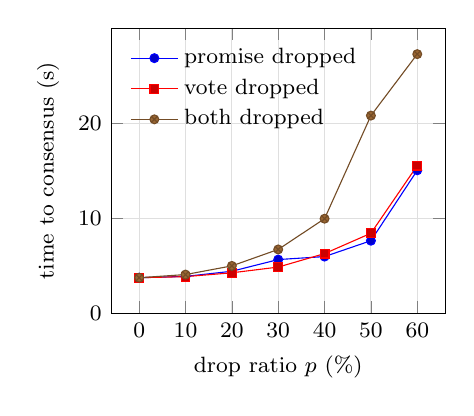
\begin{tikzpicture}
\begin{axis}[paxy, xlabel={drop ratio $p$ (\%)}, ylabel={time to consensus (s)},
             xtick={0,10,20,30,40,50,60}, legend pos=north west, ymin=0]
\addplot coordinates {(0,3.727) (10,3.865) (20,4.407) (30,5.638) (40,5.951) (50,7.621) (60,15.031)};
\addplot coordinates {(0,3.727) (10,3.841) (20,4.244) (30,4.847) (40,6.265) (50,8.405) (60,15.528)};
\addplot coordinates {(0,3.727) (10,4.059) (20,4.972) (30,6.703) (40,9.937) (50,20.786) (60,27.255)};
\legend{promise dropped, vote dropped, both dropped}
\end{axis}
\end{tikzpicture}\hfill
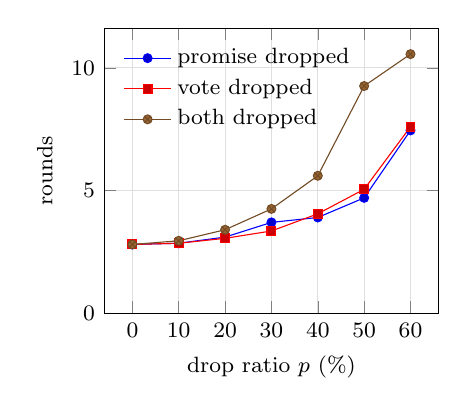
\begin{tikzpicture}
\begin{axis}[paxy, xlabel={drop ratio $p$ (\%)}, ylabel={rounds},
             xtick={0,10,20,30,40,50,60}, legend pos=north west, ymin=0]
\addplot coordinates {(0,2.80) (10,2.85) (20,3.10) (30,3.70) (40,3.90) (50,4.70) (60,7.45)};
\addplot coordinates {(0,2.80) (10,2.85) (20,3.05) (30,3.35) (40,4.05) (50,5.05) (60,7.60)};
\addplot coordinates {(0,2.80) (10,2.95) (20,3.40) (30,4.25) (40,5.60) (50,9.26) (60,10.56)};
\legend{promise dropped, vote dropped, both dropped}
\end{axis}
\end{tikzpicture}
\caption{Lost messages (mean over the trials that reached consensus within 60\,s).}
\label{fig:drop}
\end{figure}

\begin{table}[H]
\centering
\begin{tabular}{rccccc}
\toprule
& \multicolumn{3}{c}{consensus within 60\,s} & \multicolumn{2}{c}{both dropped} \\
\cmidrule(lr){2-4}\cmidrule(lr){5-6}
drop ratio $p$ & promise & vote & both & max rounds & $P(\text{ballot succeeds})$ \\
\midrule
10\% & 20/20 & 20/20 & 20/20 & 3  & 0.98 \\
20\% & 20/20 & 20/20 & 20/20 & 5  & 0.89 \\
30\% & 20/20 & 20/20 & 20/20 & 7  & 0.70 \\
40\% & 20/20 & 20/20 & 20/20 & 11 & 0.47 \\
50\% & 20/20 & 19/20 & 19/20 & 13 & 0.25 \\
60\% & 20/20 & 20/20 & 9/20  & 13 & 0.10 \\
\bottomrule
\end{tabular}
\caption{Trials (out of 20) that reached consensus, and the probability that a single uncontended ballot gets a quorum of 3 out of 5 replies in both phases.}
\label{tab:drop}
\end{table}

\textbf{Question.} Losing messages never compromises safety (every trial agreed on one value). It only hurts liveness: a lost reply costs a timeout and possibly a new round. Up to 10\% loss there is almost no visible effect, because 5 acceptors give 2 spare replies per phase. From there the number of rounds and the time grow faster and faster, and dropping both kinds of message hurts much more than dropping one, since a ballot must survive \emph{two} quorums. With 5 acceptors the probability that a single ballot succeeds is 0.70 at 30\%, 0.25 at 50\% and 0.10 at 60\% (Table~\ref{tab:drop}).

In theory consensus remains \emph{possible} for any $p<100\%$: each ballot succeeds with non-zero probability. In practice the limit is much lower because the proposer's exponential backoff doubles after each failed ballot ($10\cdot2^{k}$\,ms). 

% After 12--13 failed rounds the random sleep can reach 20--40\,s, which is why no trial got past 13 rounds before our 60\,s limit. With our parameters, consensus is reliable up to about \textbf{40\%} loss (always within $\sim$\,10\,s on average). It starts failing at \textbf{50\%} of both messages (1 trial out of 20 missed the limit). At \textbf{60\%} of both it is no longer practical (only 9 of 20 trials decided within 60\,s, after up to 13 rounds). Dropping only one message type is tolerated up to 60\%. Beyond about 70\%, a ballot succeeds less than 3\% of the time and consensus is effectively impossible.

\subsection{Number of \textit{acceptors} and \textit{proposers}}

\textbf{Experiment.} We varied the number of acceptors (3 to 51) with 3 proposers, and the number of proposers (1 to 20) with 5 acceptors. Figure~\ref{fig:scale} shows both, for the basic proposer and for the improved one of Section~\ref{sec:improvement}. All trials reached consensus.

\begin{figure}[H]
\centering
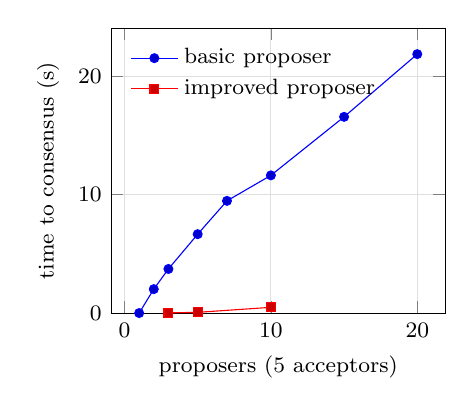
\begin{tikzpicture}
\begin{axis}[paxy, xlabel={proposers (5 acceptors)}, ylabel={time to consensus (s)},
             legend pos=north west, ymin=0]
\addplot coordinates {(1,0.006) (2,2.026) (3,3.727) (5,6.663) (7,9.474) (10,11.625) (15,16.563) (20,21.856)};
\addplot coordinates {(3,0.023) (5,0.068) (10,0.490)};
\legend{basic proposer, improved proposer}
\end{axis}
\end{tikzpicture}\hfill
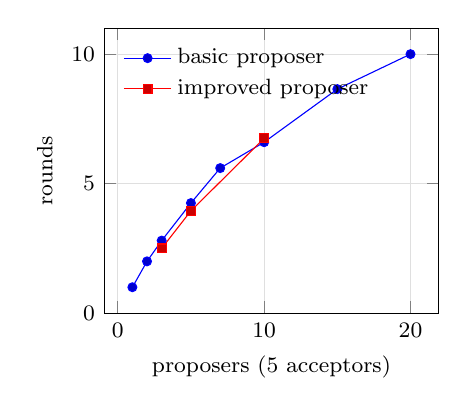
\begin{tikzpicture}
\begin{axis}[paxy, xlabel={proposers (5 acceptors)}, ylabel={rounds},
             legend pos=north west, ymin=0]
\addplot coordinates {(1,1.00) (2,2.00) (3,2.80) (5,4.25) (7,5.60) (10,6.60) (15,8.65) (20,10.00)};
\addplot coordinates {(3,2.50) (5,3.95) (10,6.75)};
\legend{basic proposer, improved proposer}
\end{axis}
\end{tikzpicture}

\vspace{6pt}
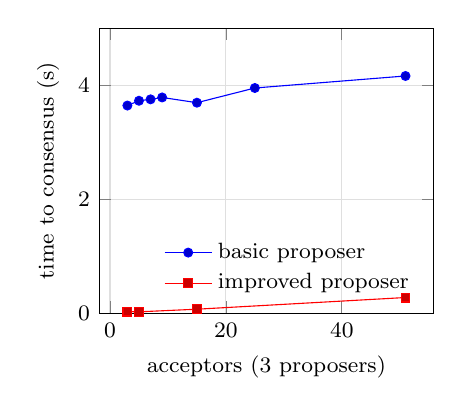
\begin{tikzpicture}
\begin{axis}[paxy, xlabel={acceptors (3 proposers)}, ylabel={time to consensus (s)},
             legend pos=south east, ymin=0, ymax=5]
\addplot coordinates {(3,3.643) (5,3.727) (7,3.752) (9,3.785) (15,3.693) (25,3.951) (51,4.162)};
\addplot coordinates {(3,0.027) (5,0.023) (15,0.069) (51,0.274)};
\legend{basic proposer, improved proposer}
\end{axis}
\end{tikzpicture}\hfill
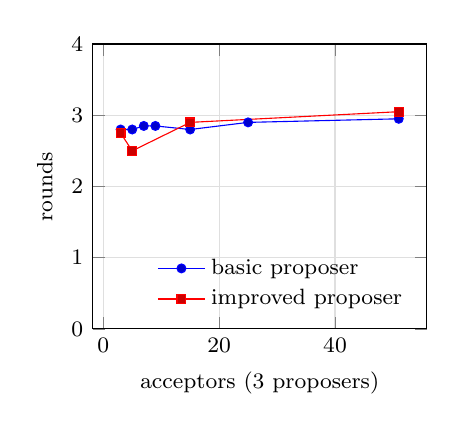
\begin{tikzpicture}
\begin{axis}[paxy, xlabel={acceptors (3 proposers)}, ylabel={rounds},
             legend pos=south east, ymin=0, ymax=4]
\addplot coordinates {(3,2.80) (5,2.80) (7,2.85) (9,2.85) (15,2.80) (25,2.90) (51,2.95)};
\addplot coordinates {(3,2.75) (5,2.50) (15,2.90) (51,3.05)};
\legend{basic proposer, improved proposer}
\end{axis}
\end{tikzpicture}
\caption{Scaling the number of proposers (top) and acceptors (bottom).}
\label{fig:scale}
\end{figure}

\textbf{Question.} \emph{More acceptors, same proposers.} The number of rounds barely changes (2.8 with 3 acceptors, 2.95 with 51): rounds are caused by \emph{contention between proposers}, and that does not depend on how many acceptors there are. The time grows slowly, because each phase has to send and receive more messages (and each acceptor writes its state to disk). The benefit is \emph{fault tolerance}: with $N$ acceptors and a quorum of $\lfloor N/2\rfloor+1$, Paxos tolerates $\lfloor (N-1)/2\rfloor$ crashed or unreachable acceptors (1 with 3, 2 with 5, 25 with 51). The cost is \emph{message traffic}: one ballot sends $N$ \texttt{prepare}, up to $N$ \texttt{promise}/\texttt{sorry}, $N$ \texttt{accept} and up to $N$ \texttt{vote}/\texttt{sorry}, i.e.\ about $4N$ messages per ballot, so traffic grows linearly with $N$.

\emph{More proposers, same acceptors.} The rounds grow roughly linearly with the number of proposers (1 round with a single proposer, 4.25 with 5, 10 with 20). Proposers pre-empt each other: each new \texttt{prepare} with a higher round invalidates the promises another proposer is collecting, and the loser retries with a higher round, pre-empting someone else (the duelling-proposers problem of Paxos). The randomised backoff is what eventually breaks the symmetry. More proposers do not improve fault tolerance for safety, but they make progress more likely if some proposers crash. This is why real systems elect a single \emph{leader} (distinguished proposer).

\subsection{Distributed execution}

\textbf{Code.} The \texttt{acceptor} and \texttt{proposer} modules are unchanged. Only \texttt{paxy} changes, with a new \texttt{start\_dist/1} and \texttt{stop\_dist/0} (the local \texttt{start/1} is kept). The changes are:

\begin{enumerate}
\item The Erlang runtime is started as named nodes sharing a cookie, e.g.\ \texttt{erl -sname paxy-acc -setcookie paxy} and \texttt{erl -sname paxy-pro -setcookie paxy}. \texttt{start\_dist} is called from a third node (or either of them), which hosts the GUI. It builds the full node names from its own host and first checks with \texttt{net\_adm:ping} that both nodes are reachable.
\item The acceptors are created \emph{on} \texttt{paxy-acc}: we \texttt{spawn(AccNode, Fun)} a process there that runs the original \texttt{start\_acceptors/2}. Since \texttt{register/2} is local to the calling node, the names \texttt{homer}, \dots, \texttt{maggie} are registered locally on \texttt{paxy-acc}, as required.
\item That process replies \texttt{acceptors\_ready} only after all acceptors are registered, and \texttt{start\_dist} waits for it, so the proposers are created only once the acceptors are up and running.
\item The proposers are created on \texttt{paxy-pro} (again with \texttt{spawn(ProNode, Fun)} and the original \texttt{start\_proposers/5}). The only difference is that they receive the acceptors as remote names, \texttt{\{homer, 'paxy-acc@host'\}}, which \texttt{!} (and our \texttt{send/2}) accept directly. GUI panels and the waiting process are plain pids, which work across nodes transparently.
\item \texttt{stop\_dist/0} sends \texttt{stop} to every \texttt{\{Name, AccNode\}}. It waits (with \texttt{erlang:monitor} on the remote names) until they have terminated before closing the GUI, because otherwise their last panel updates, which travel over the network, may reach panels that are already destroyed.
\end{enumerate}

\begin{lstlisting}
start_dist(Sleep) ->
  AccNode = node_name('paxy-acc'), ProNode = node_name('paxy-pro'),
  [pong = net_adm:ping(N) || N <- [AccNode, ProNode]],
  {AccIds, PropIds} = start_gui(),
  Self = self(),
  spawn(AccNode, fun() -> start_acceptors(AccIds, ?AccRegister),
                          Self ! acceptors_ready end),
  receive acceptors_ready -> ok end,
  Acceptors = [{Name, AccNode} || Name <- ?AccRegister],
  spawn(fun() ->
    Waiter = self(),
    spawn(ProNode, fun() ->
      start_proposers(PropIds, ?PropInfo, Acceptors, Sleep, Waiter) end),
    wait_proposers(length(PropIds)), ...
  end).
\end{lstlisting}

On our machine the short host name resolved to LAN addresses where \texttt{epmd} was not reachable (\texttt{net\_adm:ping} returned \texttt{pang}). Starting all nodes with an explicit host (\texttt{-sname paxy-acc@localhost}, \texttt{paxy-pro@localhost}, \texttt{paxy@localhost}) solved it, with no change in the code.

\textbf{Experiment.} We ran \texttt{paxy:start\_dist([500,1000,1500])} with three nodes. The acceptors registered on \texttt{paxy-acc}, the proposers ran on \texttt{paxy-pro}, and all three proposers decided the same value (red; \texttt{fry} in round 1, \texttt{bender} and \texttt{leela} in round 2). \texttt{paxy:crash\_dist(marge)} crashed and recovered an acceptor on the remote node, and \texttt{stop\_dist()} stopped everything and left no state files behind.

\noindent\textbf{Video:} \textcolor{red}{\textbf{[TODO: link to the video of the distributed execution]}}

\subsection{Fault tolerance}

\textbf{Code.} The acceptor stores \texttt{\{Promised, Voted, Value, PanelId\}} with the \texttt{pers} module (a \texttt{dets} table named after the acceptor), and the four requirements are met as follows:

\begin{enumerate}
\item \emph{Most up-to-date state on failure.} The state is written \emph{before} replying (write-ahead). A crash can therefore never lose a promise or vote that a proposer already received. The \texttt{sync} also protects against the whole Erlang node dying, not only the acceptor process.
\item \emph{Only saved when modified.} \texttt{save/5} is called only when the state changes: a new promise, or a vote for a ballot higher than \texttt{Voted}. Refusals, and votes for lower ballots, do not write. The fresh initial state is written once in \texttt{init}, so the \texttt{PanelId} is on disk even if the acceptor crashes before its first promise.
\item \emph{Removed on successful termination.} On \texttt{stop} the acceptor runs \texttt{pers:close} and \texttt{pers:delete}.
\item \emph{GUI always shows the current state.} A restarted acceptor is created with \texttt{PanelId = na}. \texttt{init(Name, na)} reads the whole state from disk, including the panel pid, and repaints the panel immediately.
\end{enumerate}

The proposer uses the fault-tolerant \texttt{send/2} of the statement (skips locally unregistered acceptors instead of raising \texttt{badarg}), and we added \texttt{crash/1} to \texttt{paxy} (and \texttt{crash\_dist/1}, which runs it on \texttt{paxy-acc} through \texttt{rpc}).

\begin{lstlisting}
init(Name, na) ->                          % restart after a crash
  pers:open(Name),
  {Promised, Voted, Value, PanelId} = pers:read(Name),
  update_gui(PanelId, Promised, Voted, Value),
  acceptor(Name, Promised, Voted, Value, PanelId);
...
    {prepare, Proposer, Round} ->
      case order:gr(Round, Promised) of
        true ->
          save(Name, Round, Voted, Value, PanelId),     % persist first
          reply(Proposer, {promise, Round, Voted, Value}, ...),
\end{lstlisting}

\textbf{Experiment.} \texttt{bench:ft\_test()} drives acceptor \texttt{homer} by hand. It promises \texttt{\{3,fry\}}, votes red in \texttt{\{3,fry\}}, and promises \texttt{\{5,leela\}}. Then it is crashed with \texttt{paxy:crash(homer)}. After the restart, \texttt{homer} printed \texttt{RECOVERED promised \{5,leela\} voted \{3,fry\} colour \{255,0,0\}}, its panel showed the same values again, it refused \texttt{prepare \{4,bender\}} (\texttt{sorry}), and it answered \texttt{prepare \{6,bender\}} with \texttt{\{promise, \{6,bender\}, \{3,fry\}, \{255,0,0\}\}}. So it recovered exactly the state it had before failing. After \texttt{stop} the state file was gone.

\noindent\textbf{Video:} \textcolor{red}{\textbf{[TODO: link to the video of a crash and recovery]}}

\subsection{Improvement based on \texttt{sorry} messages}
\label{sec:improvement}

\textbf{Code.} \texttt{collect} and \texttt{vote} get an extra argument, \texttt{Sorry}: how many more refusals can arrive before a quorum is impossible. With $N$ acceptors and quorum $Q$, at most $N-Q$ acceptors may refuse, so it starts at $N-Q+1$ (3 for 5 acceptors). Each \texttt{sorry} for the current round decrements it. When it reaches 0 the ballot aborts immediately instead of waiting for the timeout. Stale \texttt{sorry} messages from other rounds are still ignored. The clause for a reached quorum comes first, so a ballot that already has its quorum is never aborted. The basic behaviour remains available with \texttt{-Dno\_sorry\_abort}, which sets the counter to $N+1$ (unreachable).

\begin{lstlisting}
collect(0, _, _, Proposal, _) -> {accepted, Proposal};
collect(_, _, _, _, 0) -> abort;               % quorum impossible
collect(N, Round, MaxVoted, Proposal, Sorry) ->
  receive
    ...
    {sorry, {prepare, Round}} -> collect(N, Round, MaxVoted, Proposal, Sorry-1);
    ...
\end{lstlisting}

\textbf{Experiment.}

\begin{table}[H]
\centering
\begin{tabular}{lrrrr}
\toprule
& \multicolumn{2}{c}{basic} & \multicolumn{2}{c}{improved} \\
\cmidrule(lr){2-3}\cmidrule(lr){4-5}
configuration & time (s) & rounds & time (s) & rounds \\
\midrule
5 acceptors, 3 proposers  & 3.727  & 2.80 & 0.023 & 2.50 \\
5 acceptors, 5 proposers  & 6.663  & 4.25 & 0.068 & 3.95 \\
5 acceptors, 10 proposers & 11.625 & 6.60 & 0.490 & 6.75 \\
51 acceptors, 3 proposers & 4.162  & 2.95 & 0.274 & 3.05 \\
5 / 3, both delayed $\le$\,500\,ms & 4.821 & 2.90 & 1.872 & 5.25 \\
\bottomrule
\end{tabular}
\caption{Time to consensus with and without the \texttt{sorry}-based abort (20 trials each).}
\label{tab:improvement}
\end{table}

The improvement makes consensus much faster: \textbf{160$\times$} faster in the default setting (3.7\,s to 23\,ms) and 24--100$\times$ with more proposers. Without it, a proposer pre-empted by a higher round waits the full 2\,s timeout although the refusals have already arrived. With it, the proposer detects the failure as soon as the third \texttt{sorry} arrives and retries after a short backoff. The number of rounds stays about the same (contention is unchanged), so the gain is that no time is wasted per failed round. With message delays the speed-up is smaller (2.6$\times$), and the number of rounds even grows (2.9 to 5.25). Proposers now retry so quickly that they pre-empt each other more often while slow promises are still in flight, but this still takes much less time than waiting for timeouts. As shown in Table~\ref{tab:sorry}, the improvement only helps when acceptors actually send \texttt{sorry} messages.

\section{Personal opinion}

\textcolor{red}{\textbf{[TODO: write your own opinion. Draft below, edit or replace.]}}

We found this seminar one of the most instructive of the course. Paxos is usually explained in the abstract, and filling in the missing pieces of the acceptor and the proposer made us understand why each rule exists: why a promise must report the highest voted ballot, why the proposer must adopt that value, and why voting does not change the promise. The experiments were equally useful. Seeing that no amount of delay or message loss ever produced two different decisions, while the time and number of rounds grew quickly, made the difference between safety and liveness very concrete. The GUI helps a lot to follow the algorithm. The distributed and fault-tolerance parts connect the exercise with how real systems are deployed. We think it should be kept in next year's course.

\end{document}
